\section{Fibre Mat Production}
\label{sec:Fibre Mat Production}

The scintillating fibre mats are the active component of the SciFi Tracker and must be assembled very precisely and with high quality. Single scintillating fibres with a \SI{250}{\micro\metre} diameter are arranged to six layer fibre mats to receive a sufficient light yield at the photodectector. To produce these mats, the scintillating fibres are wound on a wheel with $\approx$\SI{1}{\metre} diametre. A machine has been developed to produce these mats, controlling the speed, tension and winding of the fibre onto the wheel (see Fig. \ref{fig:SciFi:WindingMachine})
 \begin{figure}[htb]
       \begin{center}
         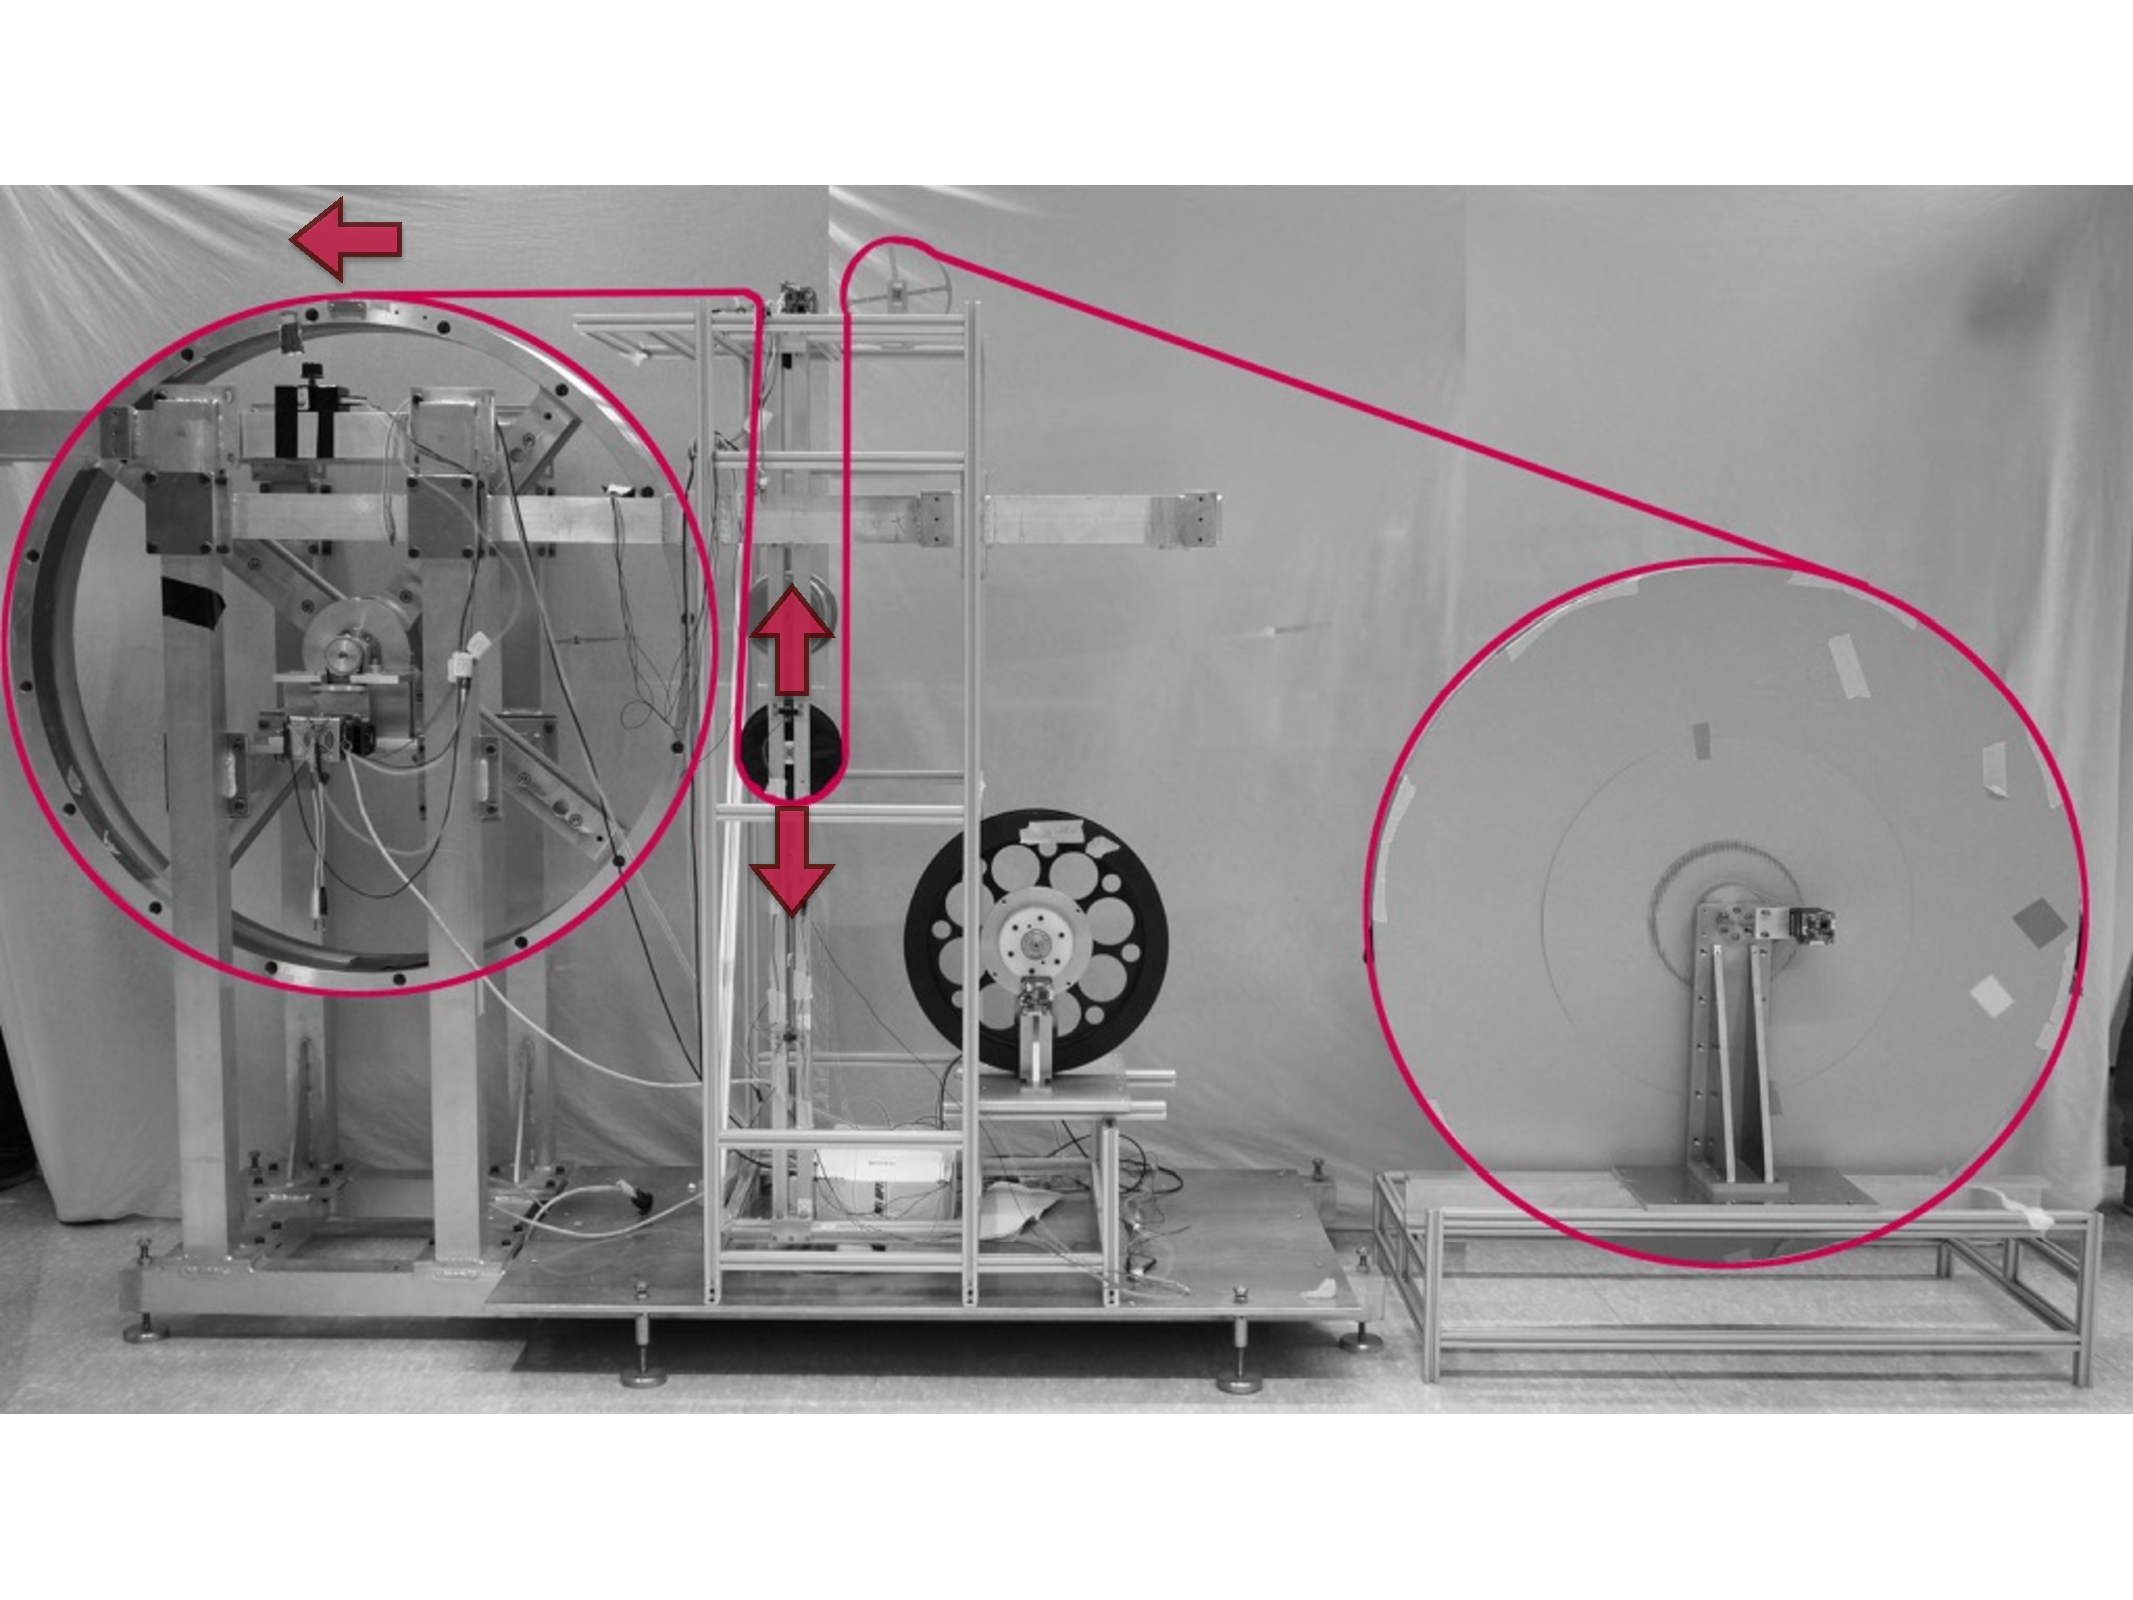
\includegraphics[width=0.75\linewidth]{figs/windingmachine}
%         \vspace*{-0.5cm}
       \end{center}
		\caption[Prototype of a winding machine to produce scintillating fibre mats.]{Prototype of a winding machine to produce scintillating fibre mats. The fibre is provided by a feeding spool (right) and moves over a loose spool to the winding wheel. The loose spool defines the tension of the fibre and regulates the speed of the feeding spool. A small spool is moving along the width of the winding wheel, for defining the correct position of the fibre.}
      	\label{fig:SciFi:WindingMachine}
   \end{figure}
   
This wheel has a milled screw to guide the fibres of the first layer and guarantee the correct pitch. At the end of the layer, the fibre is cut for starting the next layer. The layers are shifted by half the horizontal pitch with respect to each other, so that the fibres of the next layer are guided by the fibres of the respective layer before. The fibre is provided by a spool of \SI{12.5}{\kilo\metre} of scintillating fibre and is pre-guided by means of a small spool which moves along the width of the winding wheel to define the position of the fibre precisely. A loose spool in between defines the tension of the fibre and regulates the speed of the feeding spool.
$\text{TiO}_2$ loaded glue (two component epoxy) is placed between the layers. After curing the mat is cut perpendicular to the fibres and taken off the wheel to be flattenend.
For more detailed informations about the fibre mat production see also \cite{FibreMatProduction}.

